\subsection{Treatment prediction}
Because only 30 data vectors were available and model \textit{Idx\_2\_3\_4\_5\_6\_skip\_20} was trained on five datasets, only 25 data vectors were available for predicting treatments. Two slightly different approaches of training was thus attempted. First, training was conducted by a 'leave-one-out' strategy where a 1D ResNet was trained on 24 data vectors and tested on the last one, while rotating which data vector was left out, and training a new model for each rotation. In the second approach, the true segmentations was included in training which would give 48 training vectors. The same leave-one-out strategy was deployed, but only the predicted segmentation would be used for testing. Each model was trained for 120 epochs, using cross entropy as loss function and Adam for optimization with a learning rate of $10^{-4}$ and with a weight decay of $0.07$. 

\begin{table}[H]
	\hspace{-2.7cm}
	\begin{tabular}{|c|c|c|c|c|c|c|c|c|c|c|c|c|c|c|c|c|c|c|c|c|c|c|c|c|c|}
		\hline
		Idx&1
		&7
		&8
		&14
		&15
		&16
		&17
		&18
		&19
		&20
		&21
		&22
		&23
		&24
		&25
		&26
		&27
		&28
		&29
		&30
		&31
		&32
		&33
		&34
		&35\\\hline\hline
		Predictions&2
		&0
		&0
		&2
		&2
		&0
		&2
		&2
		&2
		&2
		&2
		&2
		&2
		&2
		&2
		&2
		&2
		&2
		&0
		&0
		&2
		&2
		&0
		&2
		&2\\\hline
		True&1
		&3
		&3
		&4
		&2
		&2
		&2
		&1
		&1
		&2
		&2
		&2
		&2
		&1
		&0
		&0
		&0
		&1
		&0
		&0
		&0
		&0
		&2
		&2
		&2\\\hline
	\end{tabular}
	\caption{Training a model only on the predicted segmentations, we find the following treatment predictions and true treatments shown for each video. The treatment classes are: 0 being 'healthy', 1 being 'local 5-ASA', 2 being 'Oral steroid', 3 being 'IV steroid' and 4 being 'oral 5-ASA'.}
	\label{treatmentTable}
\end{table}


\begin{figure}[H]
	\centering
	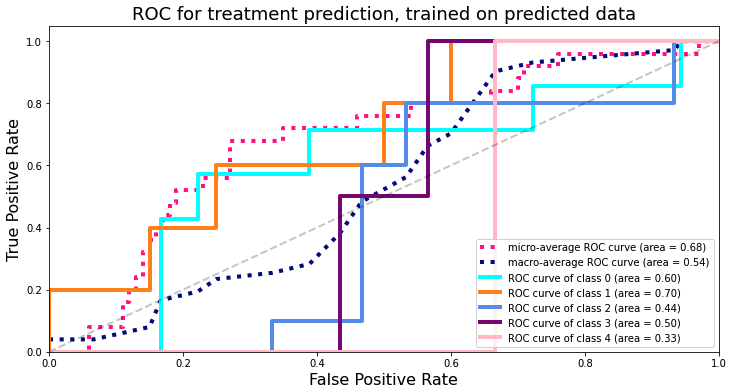
\includegraphics[width=0.85\linewidth]{Materials/Results/Treatment/RocPreds}
	\caption{ROC curves and area under the curve for the five binary 'one-vs-rest' classifiers along with micro- and macro-averages. Training was performed only on predicted segmentations.}
	\label{rocpreds}
\end{figure}
In \autoref{treatmentTable} we see the predicted treatments along the true prescribed treatment, when we train only on predicted segmentations from model \textit{Idx\_2\_3\_4\_5\_6\_skip\_20}. Computing the accuracy of this approach we get $40\%$. However, we note the model only have predicted class 2 and class 0, and there is a heavy class imbalance in the data, with only two examples of class 3 and one example of class 4.\\
It can be hard to assert the quality of a multi class classifier based on accuracy, and thus five binary 'one-vs-rest' classifiers was trained with the same parameters as the original multi class classifier. These binary models was then used to draw ROC curves for which the area under the curves could be computed. The results can be seen in \autoref{rocpreds}.

In \autoref{treatmentTableWithTrue} we see the treatment predictions and true prescribed treatment for each video for a model trained on the predicted segmentations from model \textit{Idx\_2\_3\_4\_5\_6\_skip\_20} and the true segmentations. This model was trained with the same parameters as the previous treatment prediction model. Computing the accuracy we get $48\%$, but we again note only class 0 and class 2 is predicted.
\begin{table}[H]
	\hspace{-2.7cm}
	\begin{tabular}{|c|c|c|c|c|c|c|c|c|c|c|c|c|c|c|c|c|c|c|c|c|c|c|c|c|c|}
		\hline
		Idx&1
		&7
		&8
		&14
		&15
		&16
		&17
		&18
		&19
		&20
		&21
		&22
		&23
		&24
		&25
		&26
		&27
		&28
		&29
		&30
		&31
		&32
		&33
		&34
		&35\\\hline\hline
		Predictions&2
		&0
		&0
		&2
		&2
		&2
		&2
		&2
		&2
		&2
		&2
		&2
		&2
		&2
		&2
		&2
		&2
		&2
		&0
		&0
		&2
		&0
		&0
		&2
		&2\\\hline
		True&1
		&3
		&3
		&4
		&2
		&2
		&2
		&1
		&1
		&2
		&2
		&2
		&2
		&1
		&0
		&0
		&0
		&1
		&0
		&0
		&0
		&0
		&2
		&2
		&2\\\hline
	\end{tabular}
	\caption{Training a model on both the predicted segmentations and true segmentations, we find the following treatment predictions and true treatments shown for each video. The treatment classes are: 0 being 'healthy', 1 being 'local 5-ASA', 2 being 'Oral steroid', 3 being 'IV steroid' and 4 being 'oral 5-ASA'.}
	\label{treatmentTableWithTrue}
\end{table}

In \autoref{rocpredsandtrue} ROC curves are drawn for each of the five binary 'one-vs-rest' classifiers, trained with the same parameters as the original multi class classifier and trained on both predicted and true segmentations.

\begin{figure}[H]
	\centering
	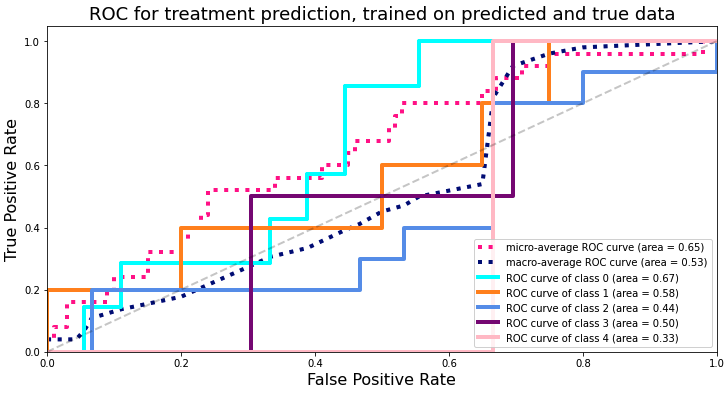
\includegraphics[width=0.85\linewidth]{Materials/Results/Treatment/RocPredsAndTrue}
	\caption{ROC curves and area under the curve for the five binary 'one-vs-rest' classifiers along with micro- and macro-averages. Training was performed on both predicted and true segmentations.}
	\label{rocpredsandtrue}
\end{figure}